\documentclass{article}
\usepackage{titlesec}
\usepackage[page]{totalcount}
\usepackage{textcomp}
\usepackage{graphicx}
\usepackage{latexsym} % diamond
\author{Chang Liu}
\title{Algorithm HW7}

\begin{document}

\newpagestyle{main}{
	\sethead{Chang Liu}{Algorithm HW7}{chang\_liu\\@student.uml.edu}
	\setfoot{}{}{\thepage \// \totalpages}
	\headrule
	\footrule
}

\pagestyle{main}

\section{Na\"{\i}ve and Speedy (15 points)}
Question: Suppose that all characters in the pattern $P$ are different. Show how to accelerate \emph{NAIVE-STRING-MATCHER} to run in time $O(n)$ on an $n$-character text $T$.

~\\
\textbf{Solution}:\newline
\indent We could use a hash-table or mapping strategy to make it less when comparing with each element of the patter P. To make it clear, before when we use the NAIVE-STRING-MATCHER algorithm, it takes $(n-m-1)*m$ time to finish it, where the $n-m-1$ is the possible compare location, and for each location, we have to compare the pattern with the text one by one, which is $m$ times.

To reduce the cost of the algorithm, if we could find a hash-mapping scheme to get a directly representation of the patter $P$, for example, mapping this string to an integer, and then for the whole text $T$, we could also get $n-m-1$ integers, and the compare between integers are constant, which is $O(1)$, and should no longer be $m$, then the whole cost of the algorithm is $O(n-m-1)$, which could be regarded as $O(n)$.

Here we could easily find the mapping scheme, according to the characters of patter $P$, each characters are different, so for a string, it is easy to map it directly to an integer. Here for pattern $P$ with the length of $m$, we could map `a' to be `1' in the first position(position is from left to right), then `b' to be `2', `c' to be `3'..., in this way once we get a new character, just use character-`a'+1 should work for all the mapping, if there are other characters unlike `a'$\sim$`z' or `A'$\sim$`Z', we still could build the map since this mapping is based on all the containing characters in text $T$. For example, string ``abc'' could be mapped directly to an integer ``123'', since they're different for each character and if we map `a' to be `1' then all others are corresponded. Similarly, the text $T$ could also be translated.

In this mapping scheme, it is constant for the mapping and the whole cost is $O(n)$.

\section{Diamonds On The Inside (15 points)}
Question: Suppose we allow the pattern $P$ to contain occurrences of a \textbf{gap character} $\Diamond$ that can match an \emph{arbitrary} string of characters (even one of zero length). For example, the pattern $ab\Diamond{ba}\Diamond{c}$ occurs in the text $cabccbacbacab$ as

\begin{center} % add this to make the figure shows in the middle of the pages
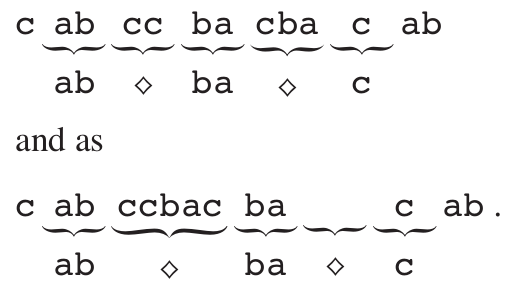
\includegraphics[scale=0.3]{hw7_p1.png} % here we could never use [] option, but it's too large, use "scale" or width=xxxin, height=xxxin to set
%\caption{EHD descriptor for distinguishing the image}
\end{center}

\noindent Note that the gap character may occur an arbitrary number of times in the pattern but not at all in the text. Give a polynomial-time algorithm to determine whether such a pattern $P$ occurs in a given text $T$ , and analyze the running time of your algorithm.

~\\
\textbf{Solution}:\newline
\indent This question could be solved using a dynamic programming problem.

1) First, for each pattern, it is divided by the $`\Diamond'{}$ characters, so we could get some substrings that are part of the original string.

2) Second, when we get the first part of the pattern $P$, for example, here $ab\Diamond{}ba\Diamond{}c$, it contains three substring which are ``ab'', ``ba'', ``c'', so we first traverse the whole original string to find the first substring ``ab''. If not found, then no match; else there is a possible match, we should find the next parts. And if we find that the next parts are not matched, we should move on and find the next possible match for the first part, because there is possibility that maybe the next substring in original string could match.

3) When we find the first match in the original string, what we need to do next is to find the remaining match. Mark the remaining string in the original string $T$ as the $T_{n-1}$, which subtracts the string from the first letter to the last matched part, so the problem could be regarded as $$ T_{n} = T_{n-1} \&\& Is\_first\_part\_matched(P_{1}) $$ here $P_{1}$ means the first part of the pattern $P$, as the example in the 2) shows ``ab''.

4) So according to the equations in the step 3), we should know that this question could be divided into many sub-questions, and if we find all the solutions of the sub-question, we could solve it, the key is to find the solution of function $Is\_first\_part\_matched(P_{i})$, which needs to be calculated by comparing the pattern part $P_{i}$ with the remaining text string $T_{n-i}$.

5) If all answers are yes, then their is a solution and the string has a match for the pattern. Otherwise, keep trying the traversing in step 2) until it find the next matches or reached the end, if it has been the end but still has no solution, then there is no match.

The overall complexity for my algorithm is $O(mn)$, because the pattern and the text both needs to be compared during this whole process, their are two loops that compare.


\section{Union of Patterns (15 points)}
Questioin: How would you extend the Rabin-Karp method to the problem of searching a text string for an occurrence of any one of a given set of $k$ patterns? Start by assuming that all $k$ patterns have the same length. Then generalize your solution to allow the patterns to have different lengths.

~\\
\textbf{Solution}:\newline
\indent The algorithms are similar to the Rabin-Karp method, except that there are many patterns that form a union.

1) For the patterns that has the \textbf{same} length: first we compute the number form of the pattern string by using the method described in the Rabin-Karp, after that we randomly select a prime number to calculate the mode. Then for the original string $T$, we also select the same length string, and using the same function to calculate the number form and divided by the prime number to get the mode. If the mode are the same, we further carefully check whether they're actually the same; If not then they're not matched, check the other strings. For any of the pattern in the pattern set, we could do the same process to check whether it contains each of the pattern.

2) For the patterns that does have \textbf{different} length: the process is quite similar except that we choose different length of strings to convert it the number form, for each pattern, we choose the same length string to covert when checking whether they're the same; since the pattern may have different length, for the check of single pattern, we should make sure that our selected substring in the original text $T$ should be the same with the current pattern length. Then check all the patterns in the pattern set.


\section{String Squared (15 points)}
Question: Show how to extend the Rabin-Karp method to handle the problem of looking for a given $m \times m$ pattern in an $n \times n$ array of characters. (The pattern may be shifted vertically and horizontally, but it may not be rotated.)

~\\
\textbf{Solution}:\newline
\indent This strategy is quite similar to the last question, except that there is more comparing because it contain a two dimensional patterns, so our focus is just to divide the $m \times m$ to some sub-strings that can be compared with the original string in the $n \times n$.

1) from the beginning to the end for the text $T$ in the column, move the pattern from left to right, so we should have $n-m$ times move.

2) from top to bottom for the text $T$ in the row, move the pattern from up to down, so we should also have $n-m$ times move.

No matter what position we're current in when the pattern moves in the text rectangle $T$, we just need the compare the $m \times m$ pattern with the $m \times m$ elements correspondingly.

To compare this $m \times m$ elements, we could divide the rectangle into $m$ rows or $m$ columns, and compare this $p_{i}$ with the corresponding string in the text at the same position. Regarding how to compare it, it is then divided into the compare the the same string, we could use the same method in question 3) and apply the Rabin-Karp method to solve it one by one.

The figure could be as follows, we just move the shadow square from left to right and from top to bottom, and compare the square with the original text string square correspondingly.

\begin{center}
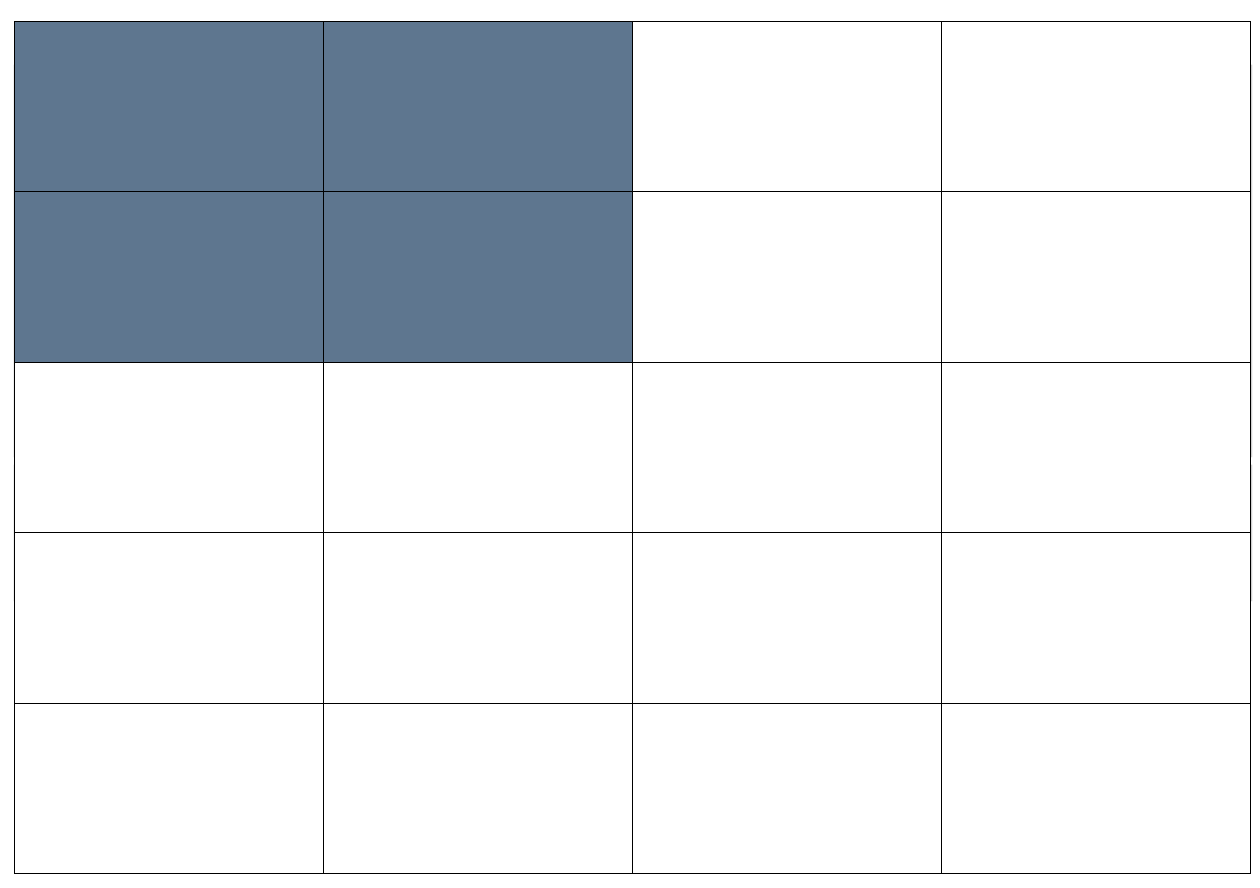
\includegraphics[scale=0.2]{hw7_1.png}
\end{center}


\section{Nothing Compares (15 points)}
Question: We call a pattern $P$ \textbf{nonoverlappable} if $P_{k} \sqsupset P_{q}$ implies $k = 0$ or $k = q$. Describe the state-transition diagram of the string-matching automaton for a nonover-lappable pattern.

~\\
\textbf{Solution}:\newline
\indent This \textbf{nonoverlappable} pattern has the property that for a sub-string of any length that are no less than 2 characters, it should not be an substring of its pattern $P$. For example, here we has a string `$abcabdef$', the first sub-string `$ab$', and the next substring `$abdef$', the first is just another part of the next, so it is not a \textbf{nonoverlappable} string.

This property shows that none of the substring should overlap with another substring of the original pattern. If we should use a state-transition diagram, then all the elements in the diagram should go back to the original start node.

Here I draw a draft graph which could describe the situation, then apart from the start and end node, all the \textbf{middle} nodes should go back to the starting node, otherwise it has an overlap of equal or more than 2 characters, that would not meet the \textbf{nonoverlappable} requirements. Regarding the last node, it doesn't have the requirement, so that it is the situation of $k = 0$ or $k = q$.

\begin{center}
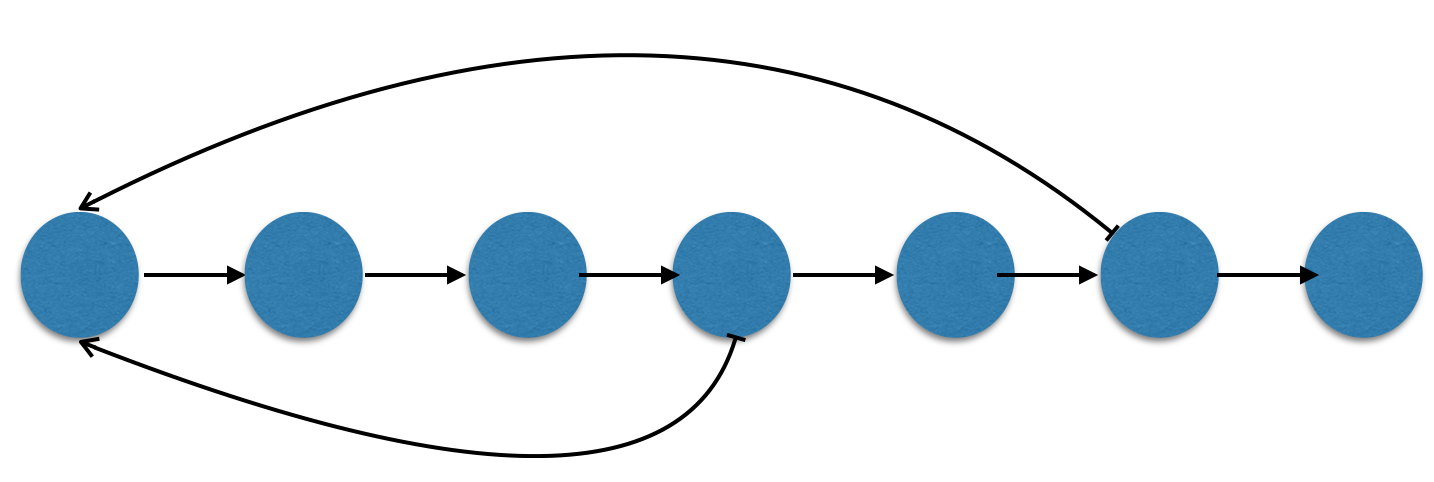
\includegraphics[scale=0.3]{hw7_2.png}
\end{center}


\section{Automaton for Diamonds (15 points)}
%\| 是双竖线,等价于 \Vert,一般是范数、模,和绝对值是两个东西。绝对值就是直接打 |x|,或者加上 \left| x \right|。其中 | 可用 \vert 代替。
Question: Given a pattern $P$ containing gap characters (see Exercise 32.1-4), show how to build a finite automaton that can find an occurrence of $P$ in a text $T$ in $O(n)$ matching time, where $n = |T|$.

~\\
\textbf{Solution}:\newline
\indent Here we know that the solution for automaton in matching is $O(n)$ once the state-transmission diagram is given, and the preprocessing time for the generating is $O(m|\Sigma|)$, m is the length of pattern, and $|\Sigma|$ is the alphabet number.

For this special pattern, since it contains `$\Diamond$', so when encountering it: 

1) we could just ignore it as it is an empty character, so draw an arrow that points to itself, meaning that it will not affect the current state.

2) Or we could see that it could also represent any number(except the whole string length) of characters, in this case, it could represent 1, 2, 3, ... characters of any alphabet in that situation, so the arrow should point to next element, next 2nd element, next 3rd element ... but we should not the the symbol should contributes to the next match, so we should only select those destionation points that lays after the symbol `$\Diamond$'. For example, string `$ab\Diamond{}cab$', then when in the 2nd node b, we should only make lines that points to the node with the character `c', \textbf{it should always point to the node that lays behind the character `$\Diamond$'}.

I draw a draft graph as follows, there is no character that states the situation of 2) but is should be clear now in my statement.

\begin{center}
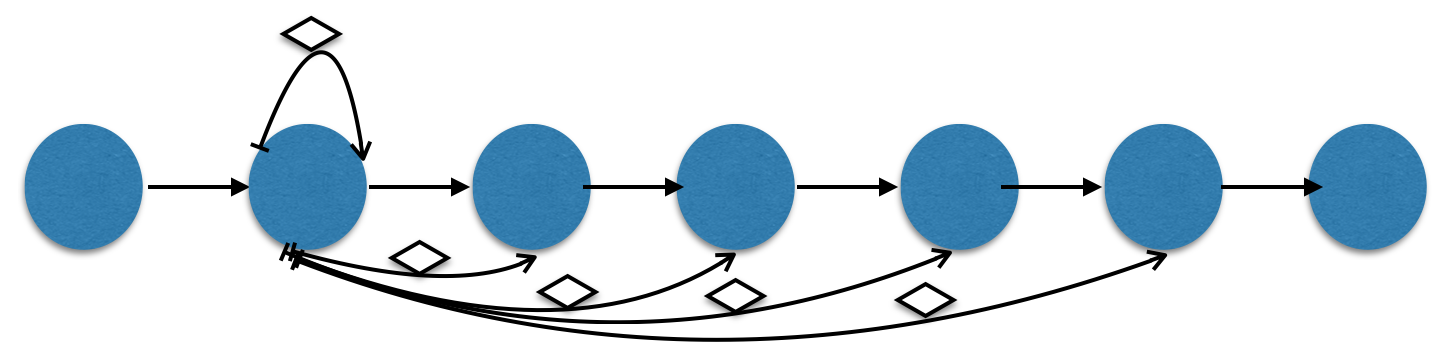
\includegraphics[scale=0.3]{hw7_3.png}
\end{center}


\section{$\pi$ is Perfect (15 points)}
Question: Explain how to determine the occurrences of pattern $P$ in the text $T$ by examining the $\pi$ function for the string $PT$ (the string of length $m+n$ that is the concatenation of $P$ and $T$).

~\\
\textbf{Solution}:\newline
\indent

\section{Cyclic Rotation (15 points)}
Question: Give a linear-time algorithm to determine whether a text $T$ is a cyclic rotation of another string $T'$ . For example, $arc$ and $car$ are cyclic rotations of each other.

~\\
\textbf{Solution}:\newline
\indent




\end{document}